\documentclass[final]{beamer}
\mode<presentation>{\usetheme{I6dv}}
\usefonttheme[onlymath]{serif}

\usepackage{microtype}
\usepackage{fixltx2e}

\usepackage[orientation=landscape,size=a1]{beamerposter} 
\usepackage{exscale}
\usepackage{booktabs, array}
\usepackage[english]{babel}
\usepackage[latin1]{inputenc}
\usepackage{amsmath,amsthm, amssymb, latexsym}
\usepackage{lipsum}
\usepackage{graphicx}
\usepackage[center,labelformat=empty, font=normal]{caption}
\usepackage[labelformat=empty, font=normal]{subcaption}

%\beamertemplategridbackground[1em]


\begin{document}
\begin{frame}{ }
    \begin{columns}[t]
        \begin{column}{.28\linewidth}

            \begin{block}{Introduction}
                \begin{itemize}
                    \item transportation forecasting model
                    \item mathematically describes the behaviour of traffic
                    \item people wish to travel on shortest path with least travel time
                    \item \alert{goal}: find a \alert{faster} algorithm for solving the \alert{shortest path} problem between origins and a destinations in transportation network
                \end{itemize}
            \end{block}

            \begin{block}{Traffic Assignment}
                \begin{itemize}
                    \item \alert{Traffic Assignment (TA)} deals with selection of \alert{shortest path} for everyone in the network to \alert{minimise} their \alert{travel times}
                    \item a \alert{non-linear} problem, travel times decrease dramatically when \alert{congestion} happens
                    \item an \alert{iterative algorithm} called \alert{Path Equilibration (PE)} algorithm is used to solve TA
                    \item \alert{PE} requires to find \alert{millions} of \alert{shortest paths}
                    \item research of using PE for TA has just begun in recent years due to its \alert{huge} computation \alert{memory} requirement
                    \item speed up TA and benefit transportation modelling
                \end{itemize}
            \end{block}

            \begin{block}{Shortest Path Algorithms}
                \begin{itemize}
                    \item find path with least distance in network
                    \item scan nodes in network in some order until destination is found
                    \item need a data structure called \alert{priority queue} to keep the scanned nodes in order so we can find the next node to scan easily
                \end{itemize}
                \begin{itemize}
                    \item in PE, can avoid shortest path calculations to speed up overall performance
                    \item first strategy: avoid the next few iterations if the shortest path of the previous two iterations are the same
                    \item second strategy: randomly avoid the next shortest path calculation in the hope that path of previous and current iteration are the same
                \end{itemize}
            \end{block}

        \end{column}
        \begin{column}{.4\linewidth}

            \begin{block}{Search Areas of Shortest Path Algorithms}
                    \vspace{2em}
                \begin{figure}
                    \centering
                    \begin{subfigure}{.5\linewidth}
                        \centering
                        {\bfseries Dijkstra's algorithm }
                        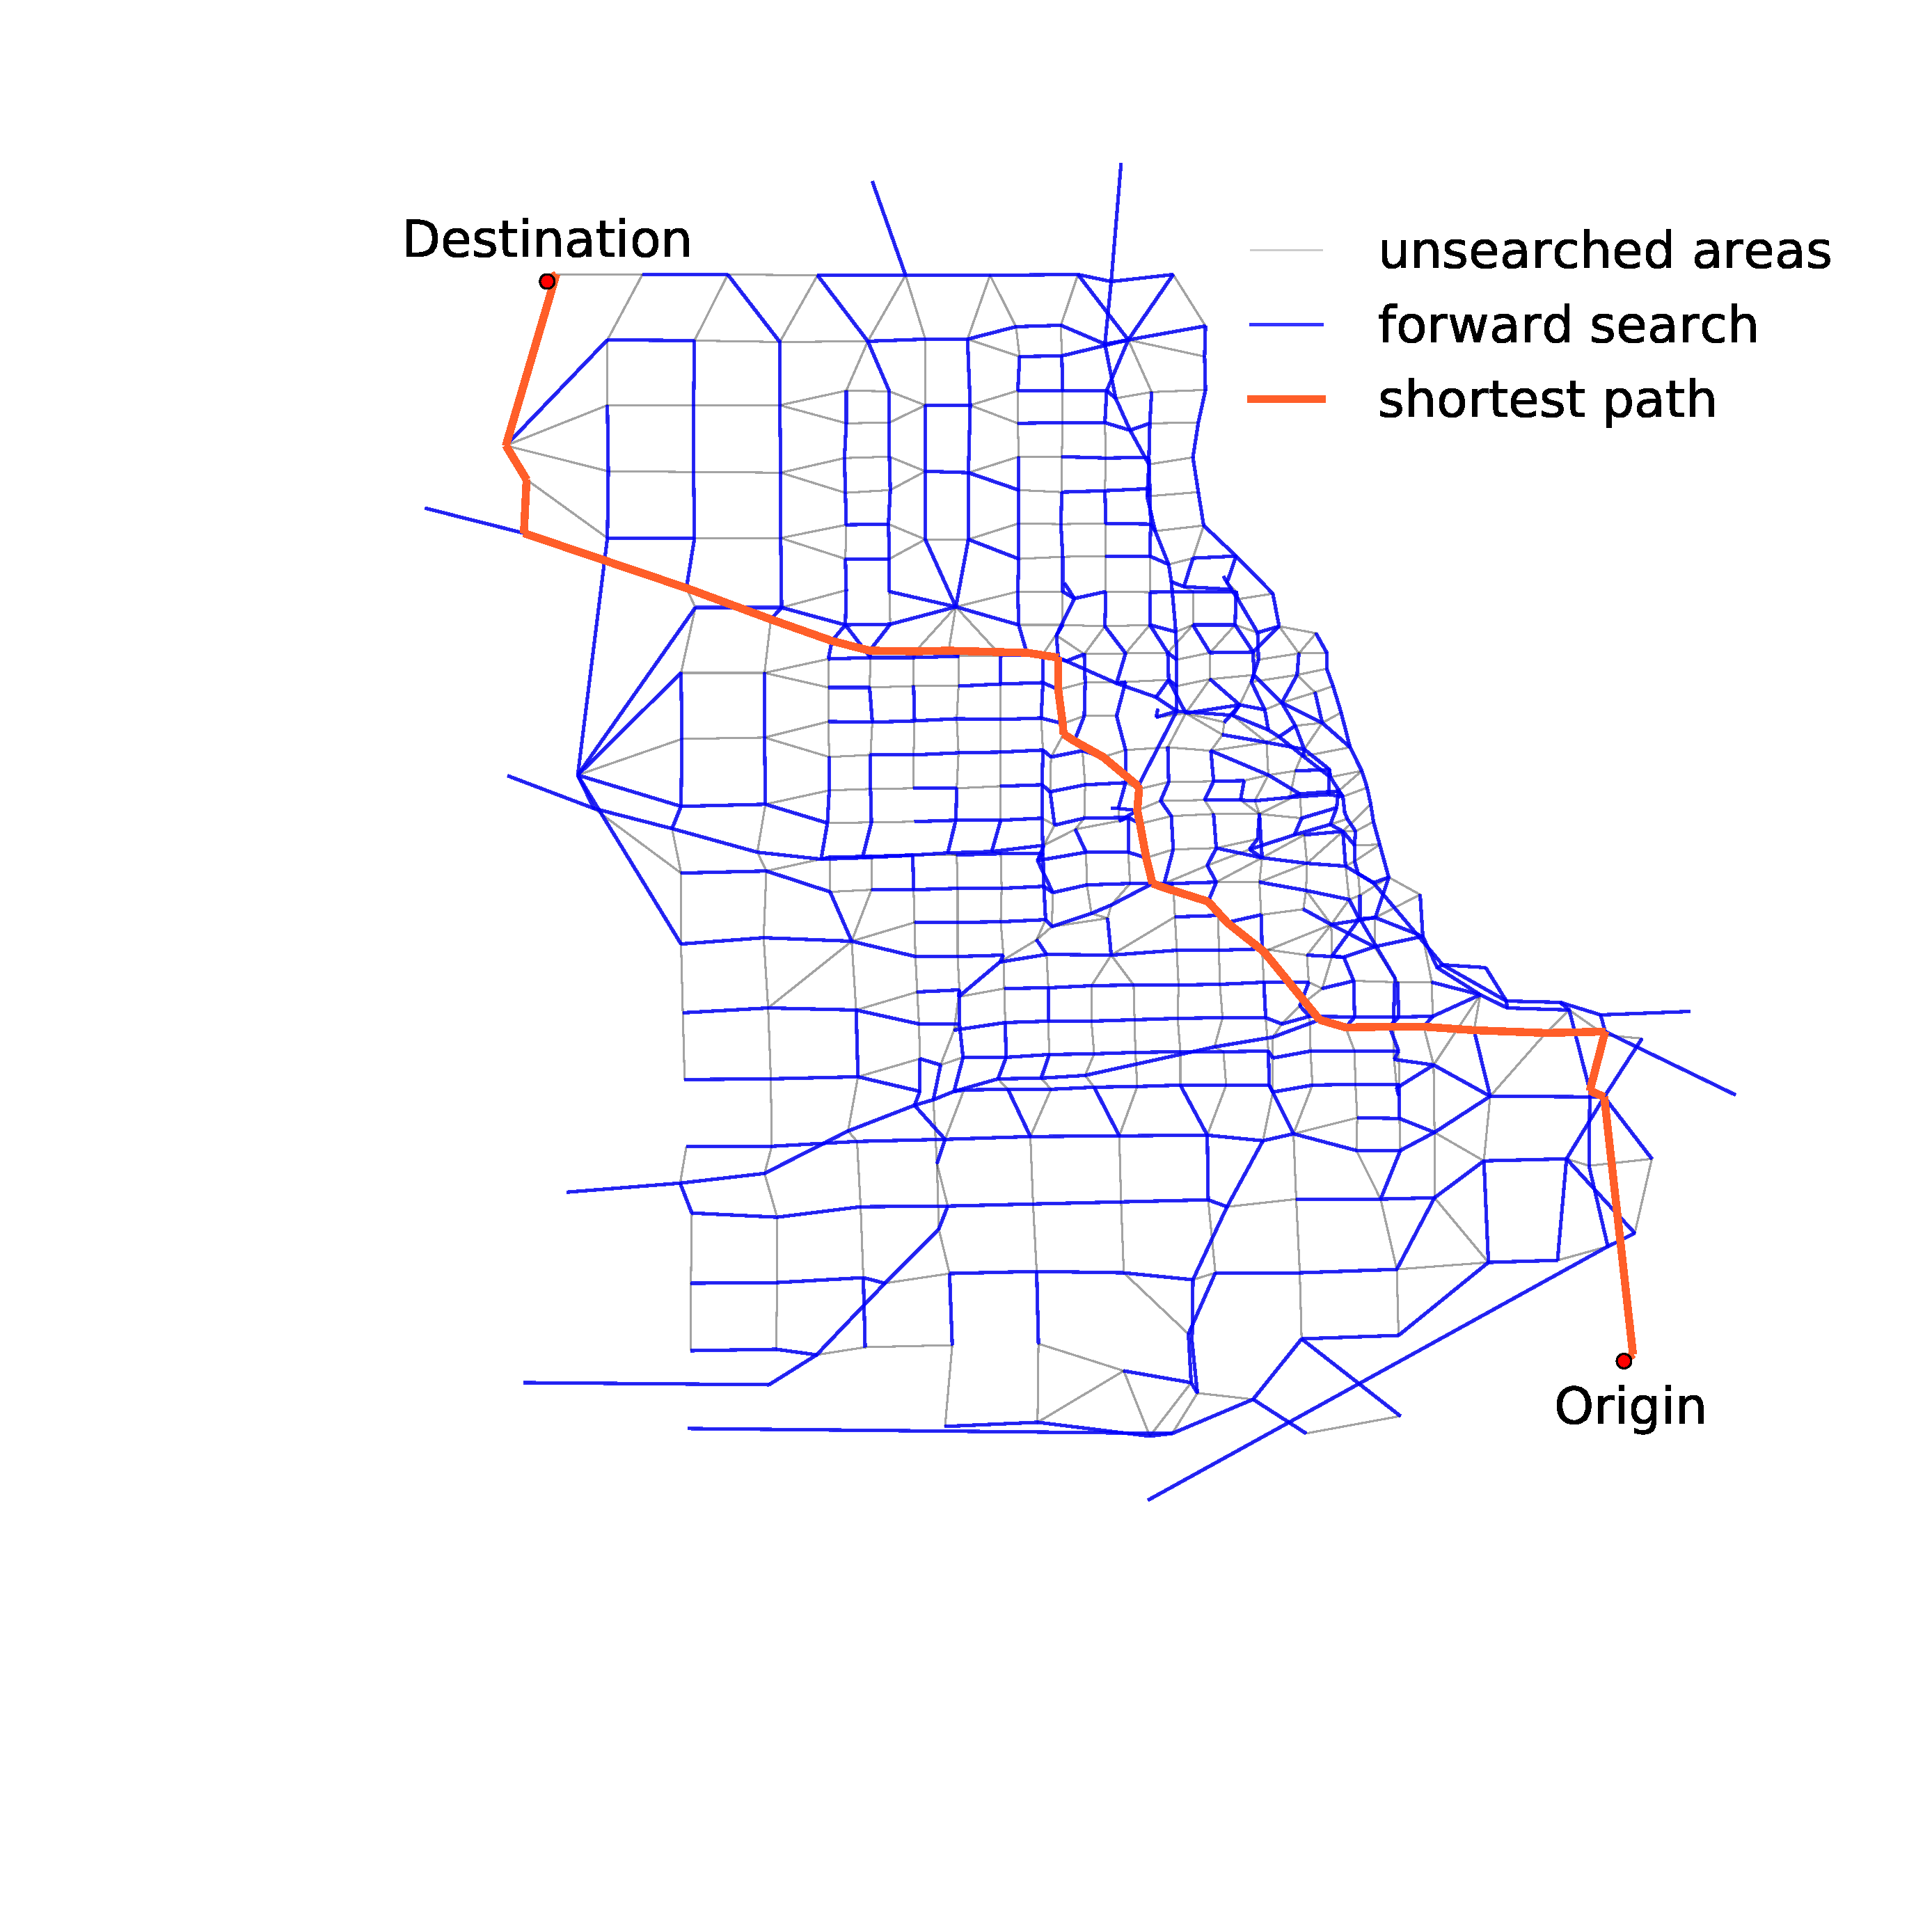
\includegraphics[width=\linewidth,trim=120px 120px 48px 60px,clip]{img/dijkstra}
                        \caption{searches the entire network}
                    \vspace{2em}
                    \end{subfigure}%
                    \begin{subfigure}{.5\linewidth}
                        \centering
                        {\bfseries Bidirectional Dijkstra's algorithm}
                        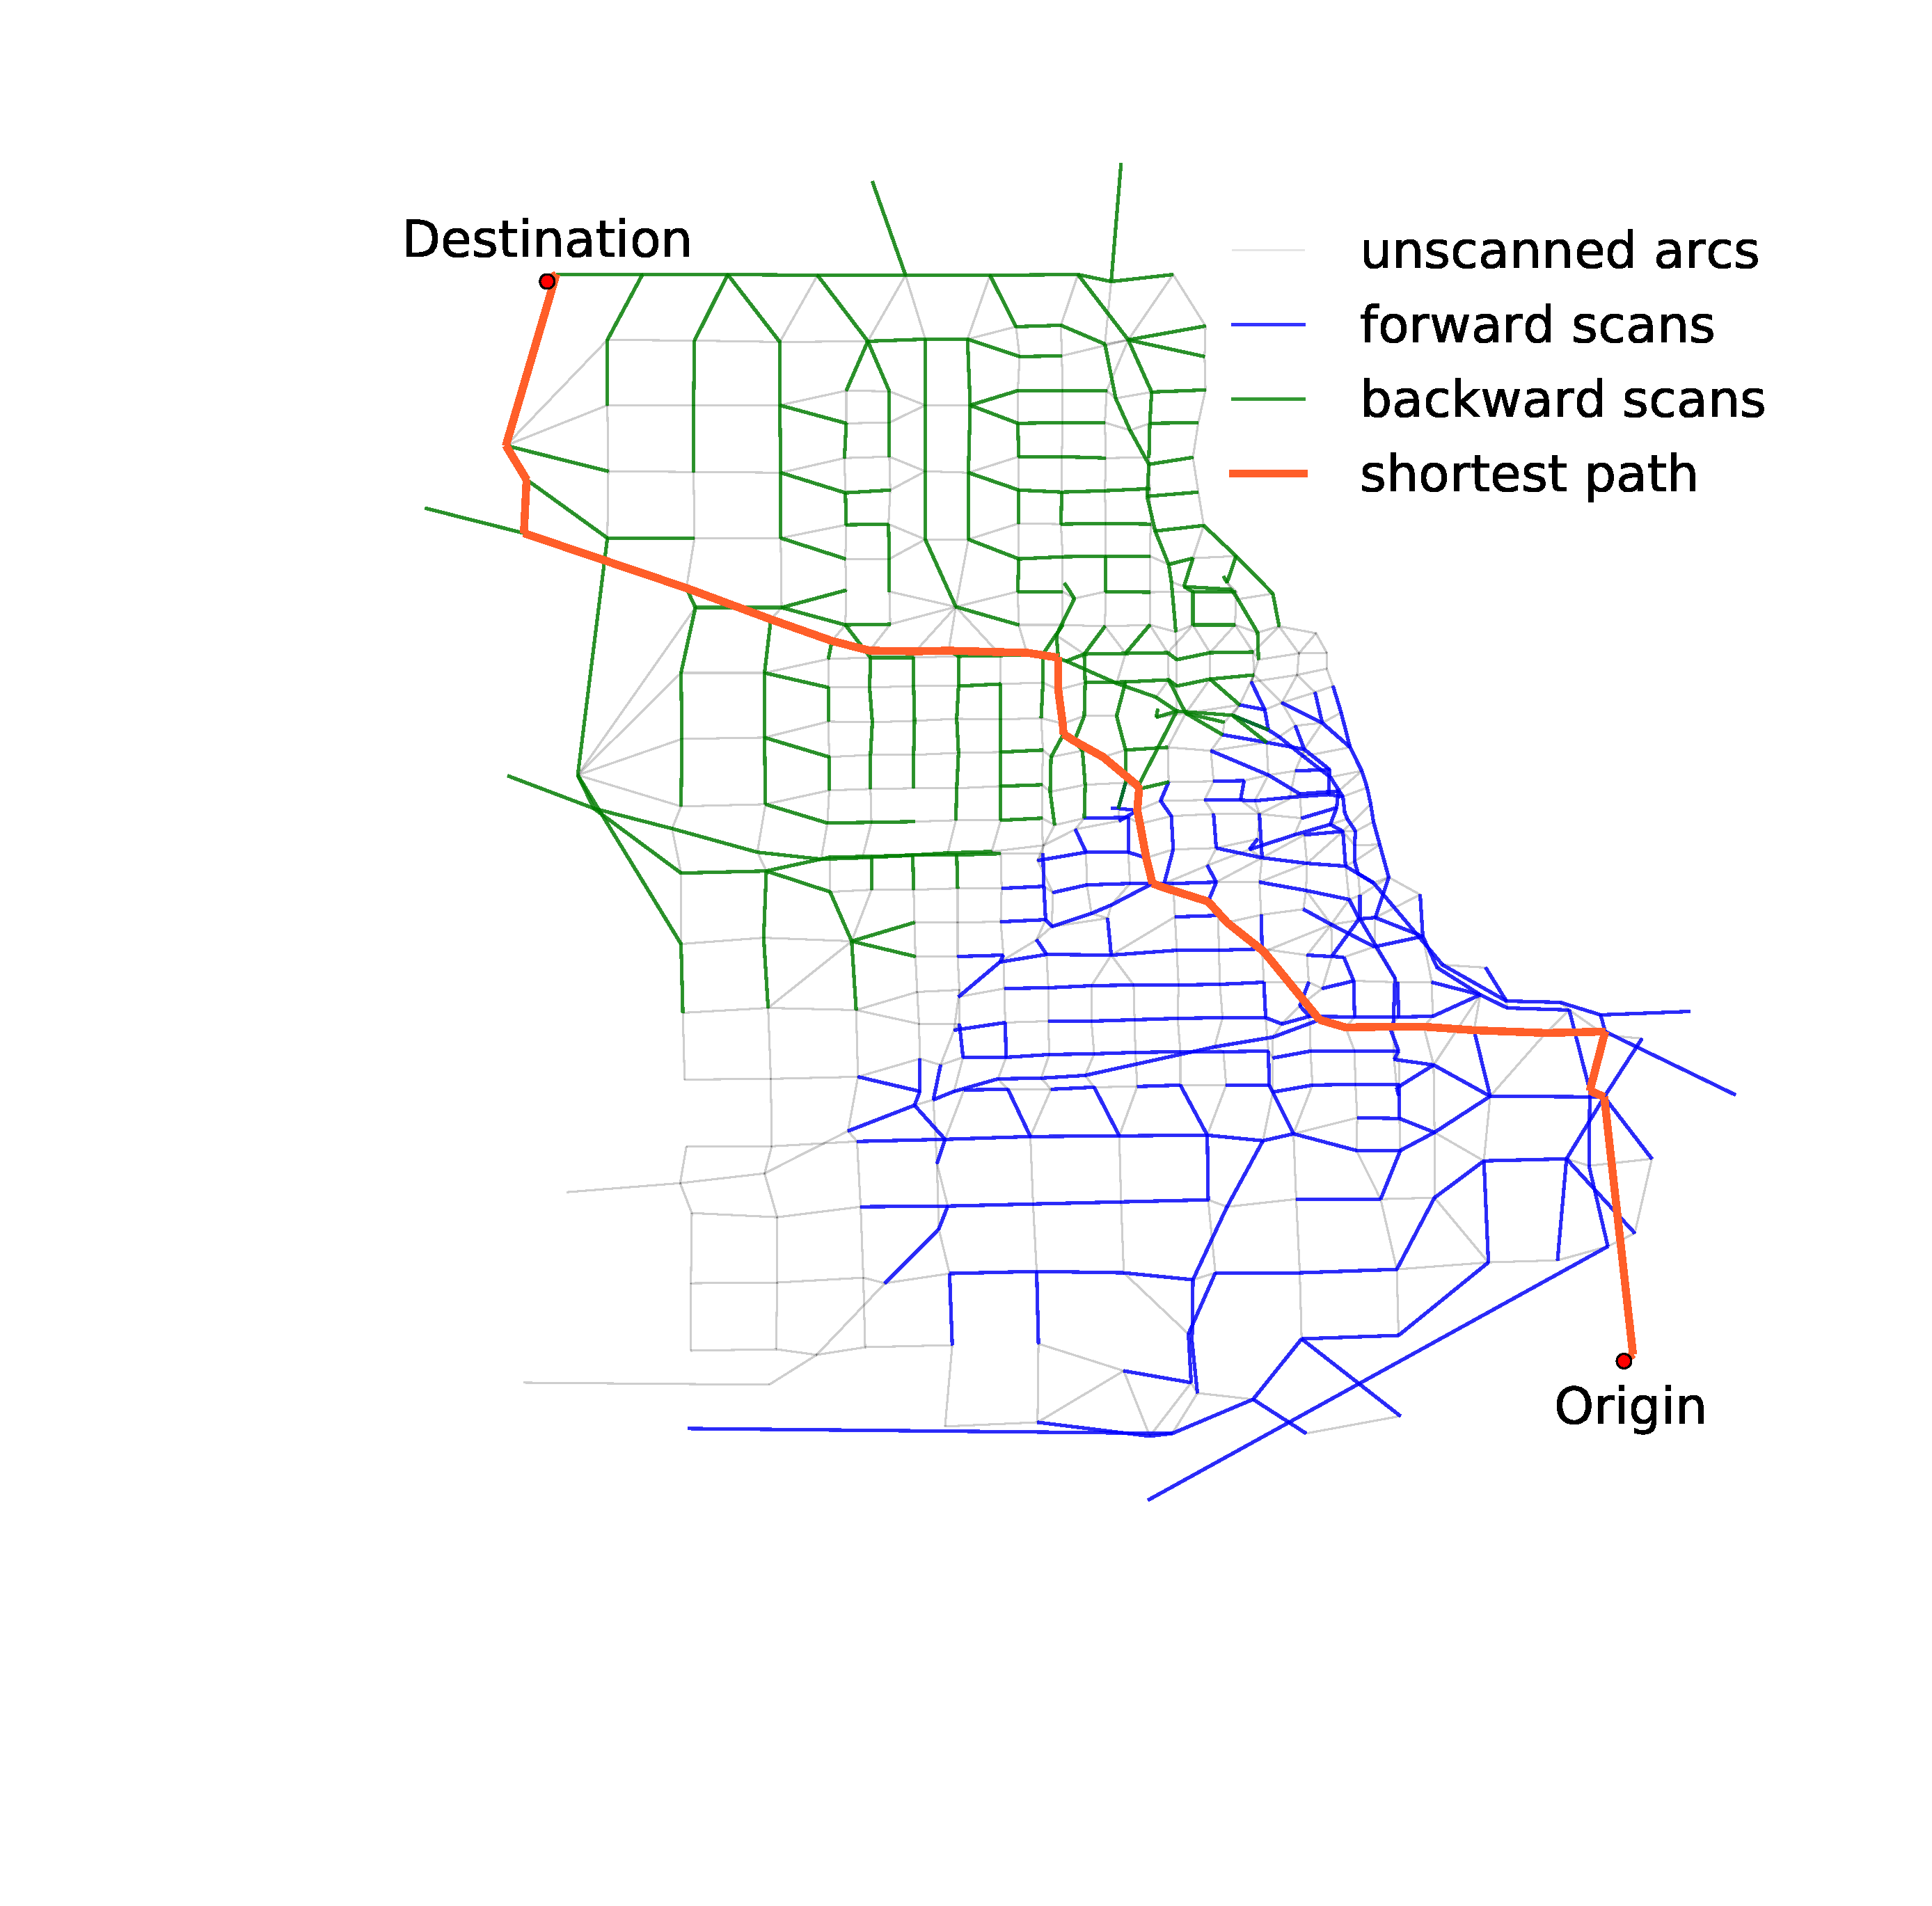
\includegraphics[width=\linewidth,trim=120px 120px 48px 60px,clip]{img/dijkstra_bidirect}
                        \caption{searches from both ends simultaneously}
                    \vspace{2em}
                    \end{subfigure}
                    \begin{subfigure}{.5\linewidth}
                        \vspace{-1.5em}
                        \centering
                        {\bfseries A* Search}
                        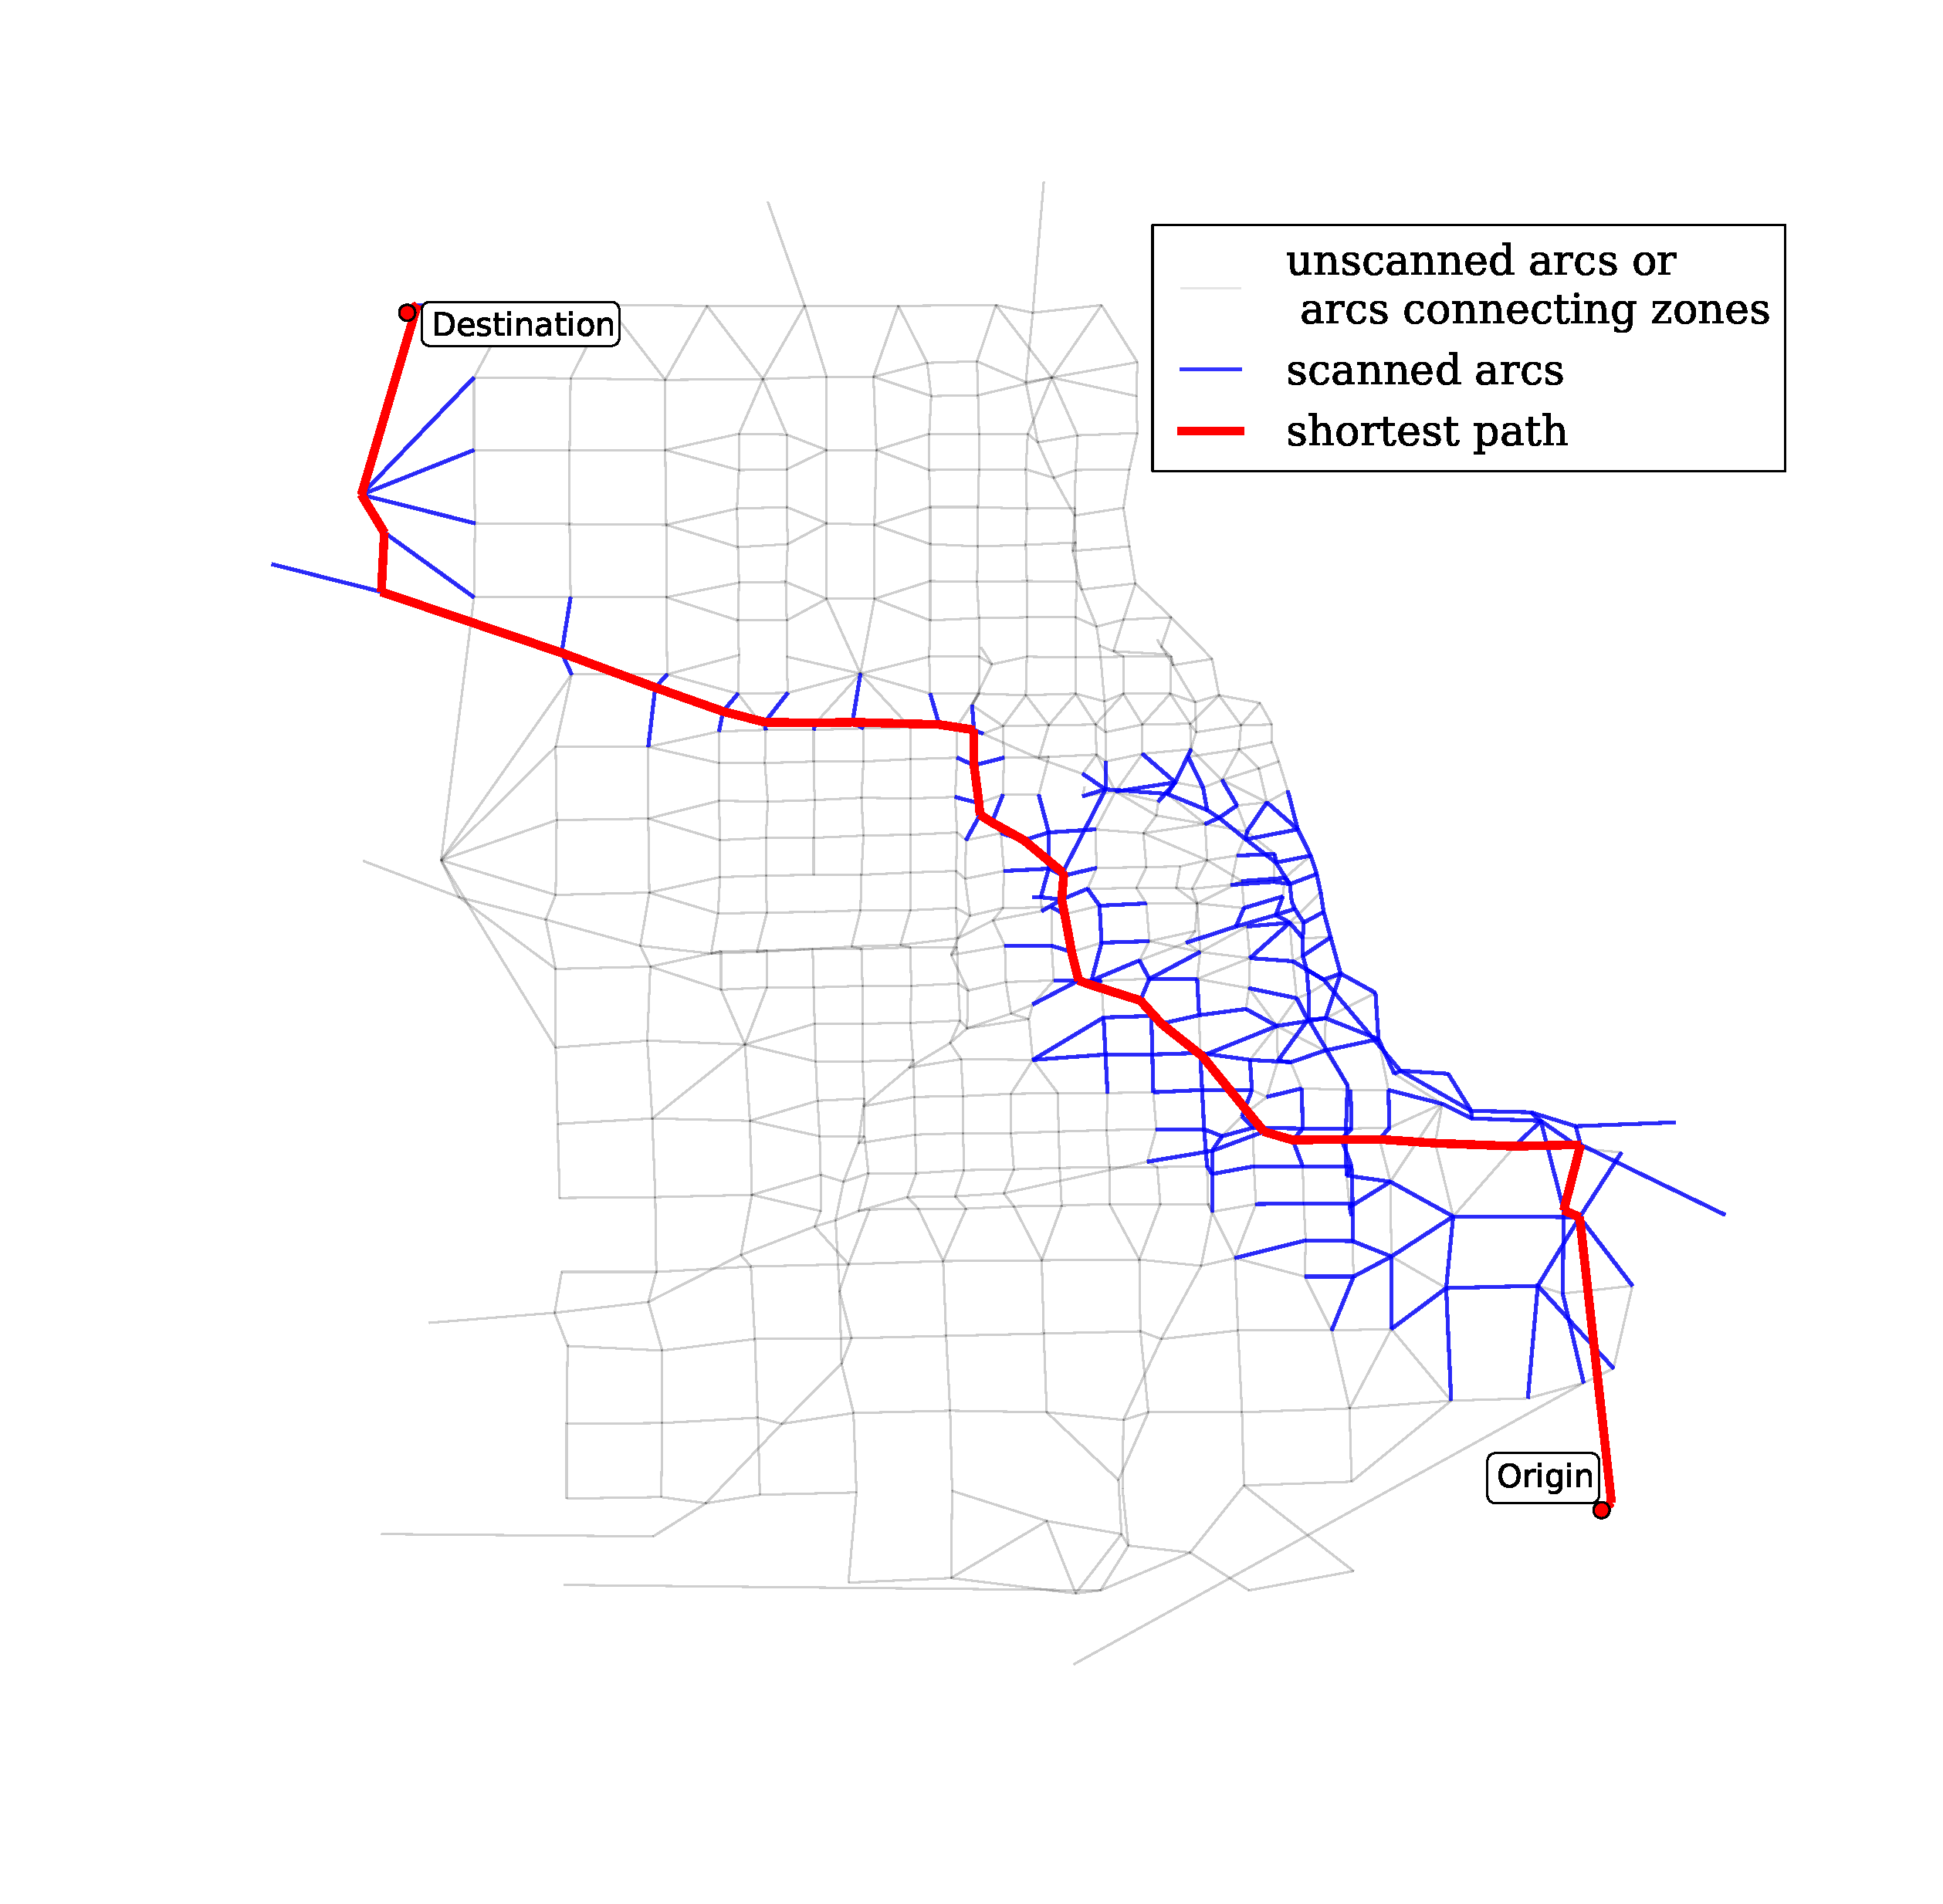
\includegraphics[width=\linewidth,trim=120px 120px 48px 60px,clip]{img/astar}
                        \caption{searches along the expected shortest path}
                    \end{subfigure}%
                    \begin{subfigure}{.5\linewidth}
                        \centering
                        {\bfseries Bidirectional A* Search}
                        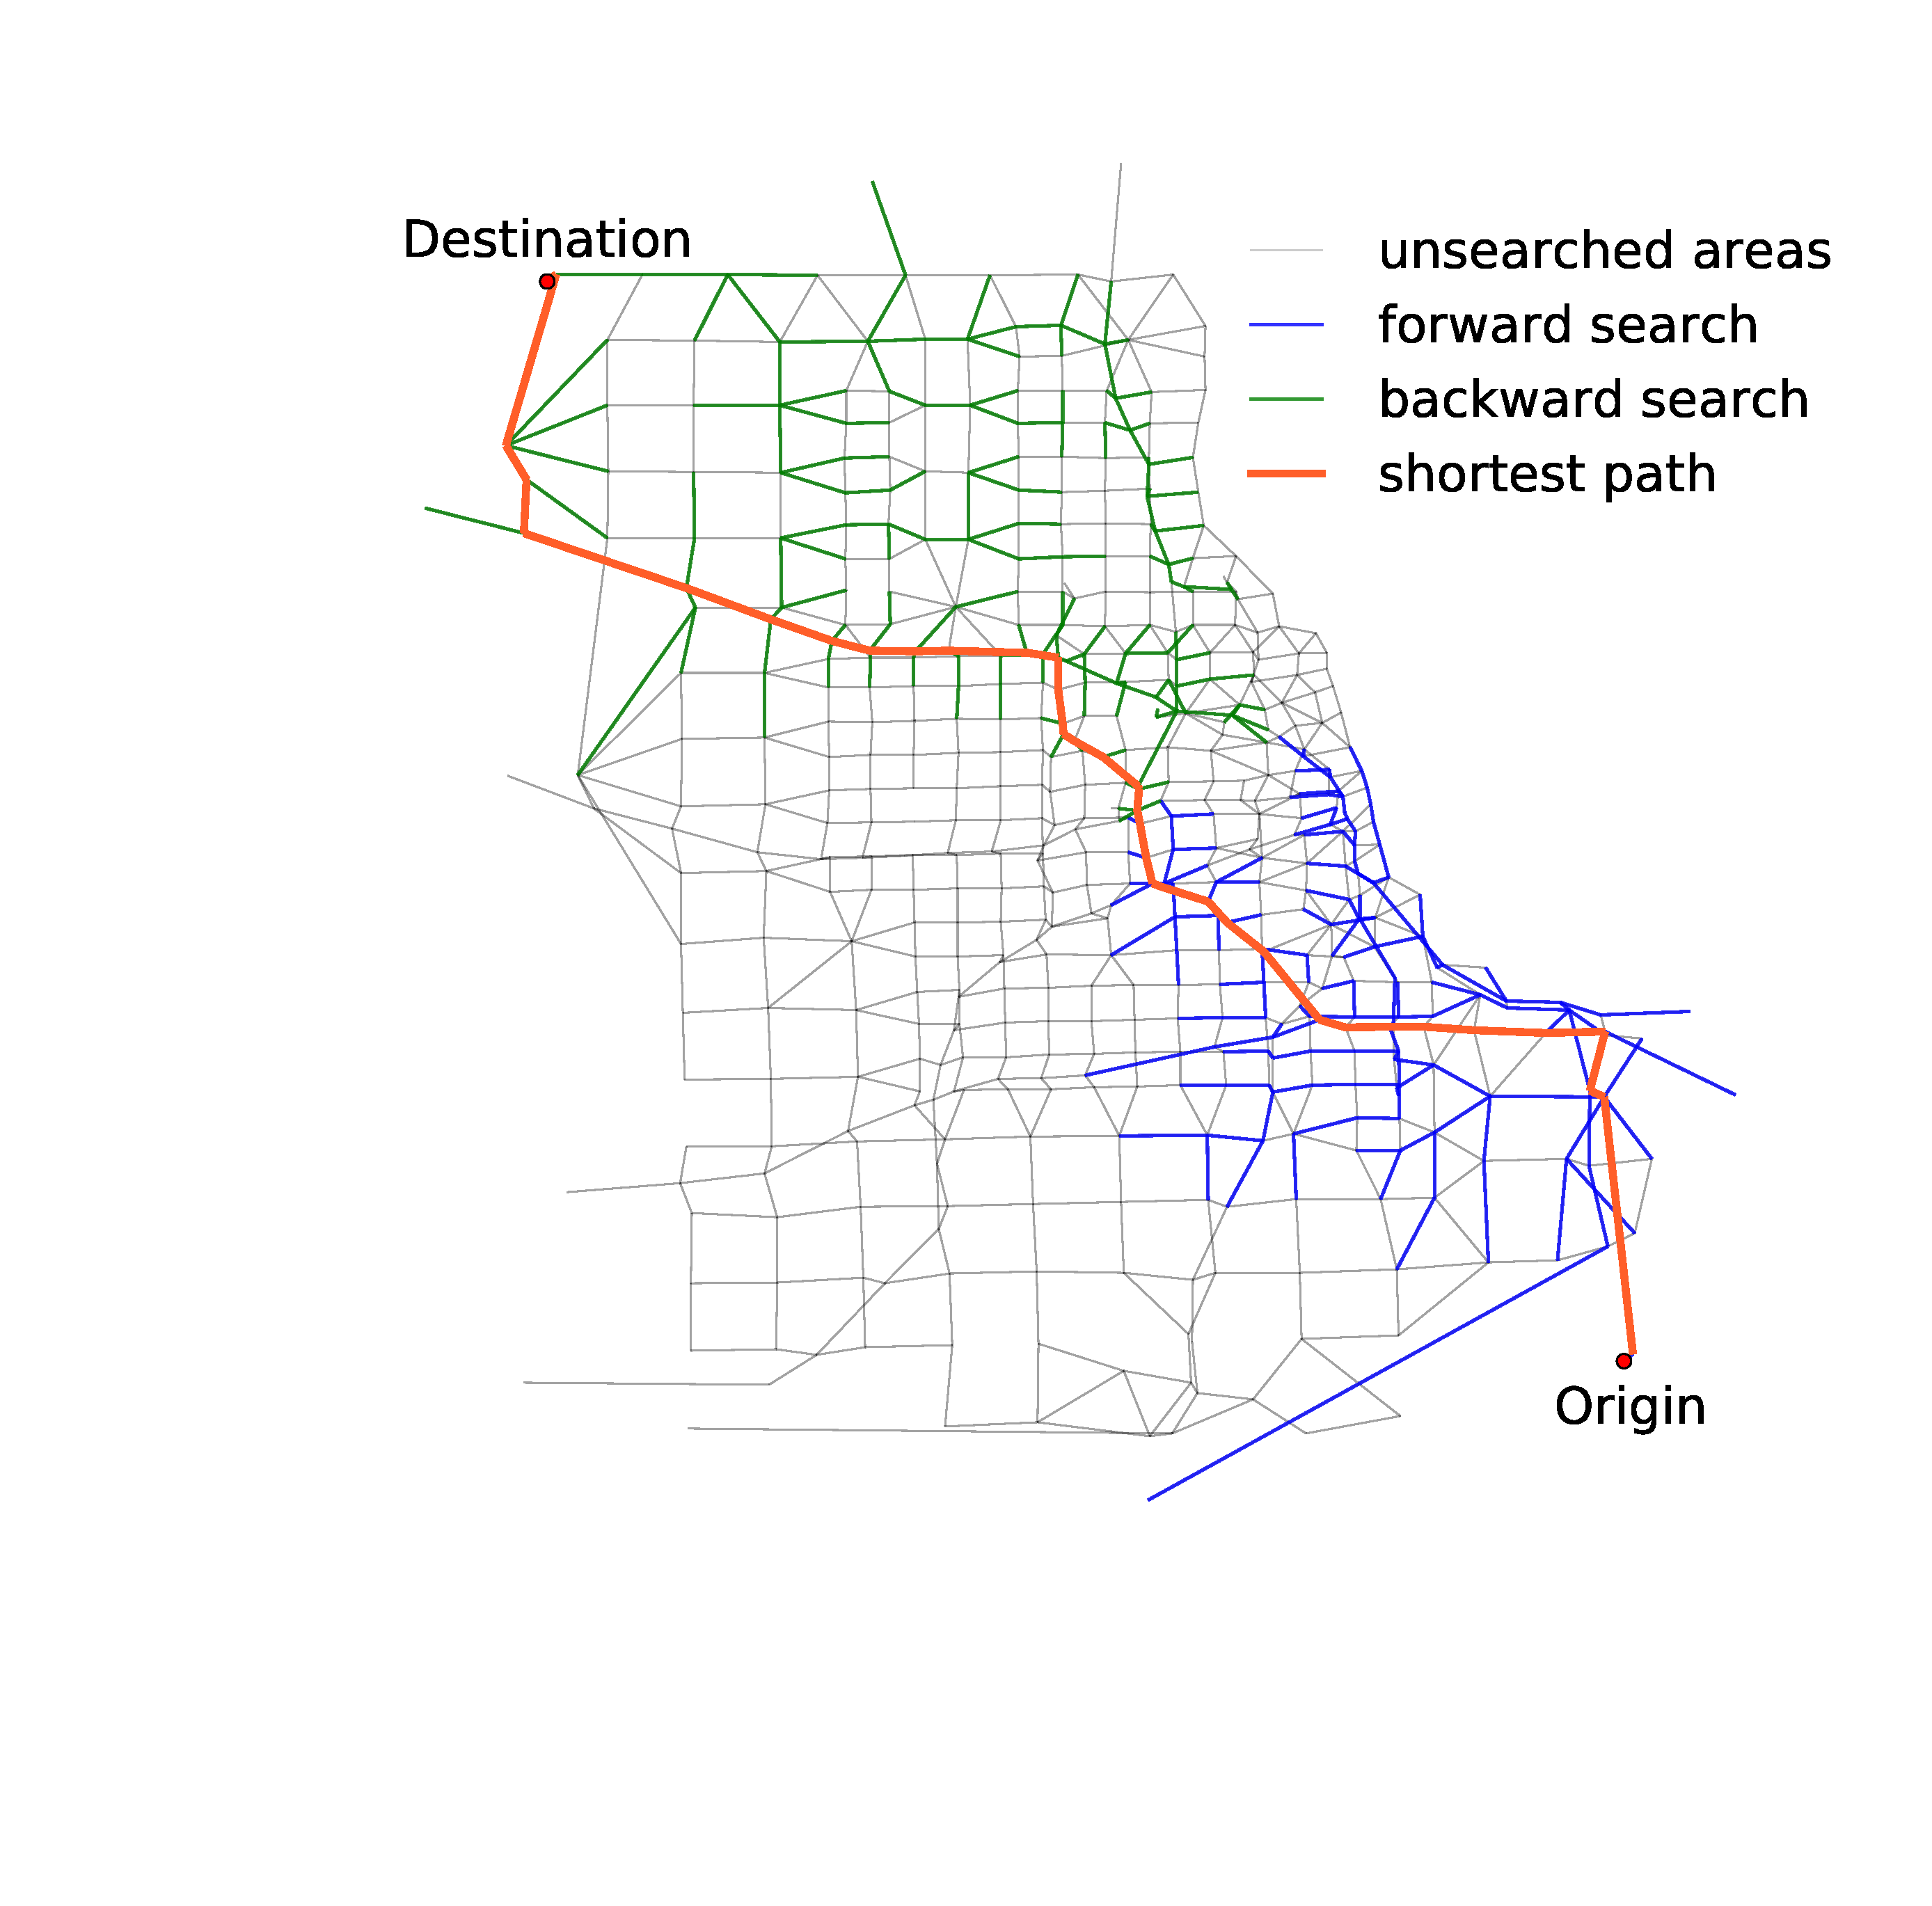
\includegraphics[width=\linewidth,trim=120px 120px 48px 60px,clip]{img/astar_bidirect}
                        \caption{searches along the expected shortest path from both ends simultaneously} 
                    \end{subfigure}
                \end{figure}
            \end{block}

        \end{column}
        \begin{column}{.28\linewidth}
            
            \begin{block}{Results}
                \begin{figure}
                    \centering
                    {\bfseries \qquad Run times of shortest path algorithms on a test network}
                    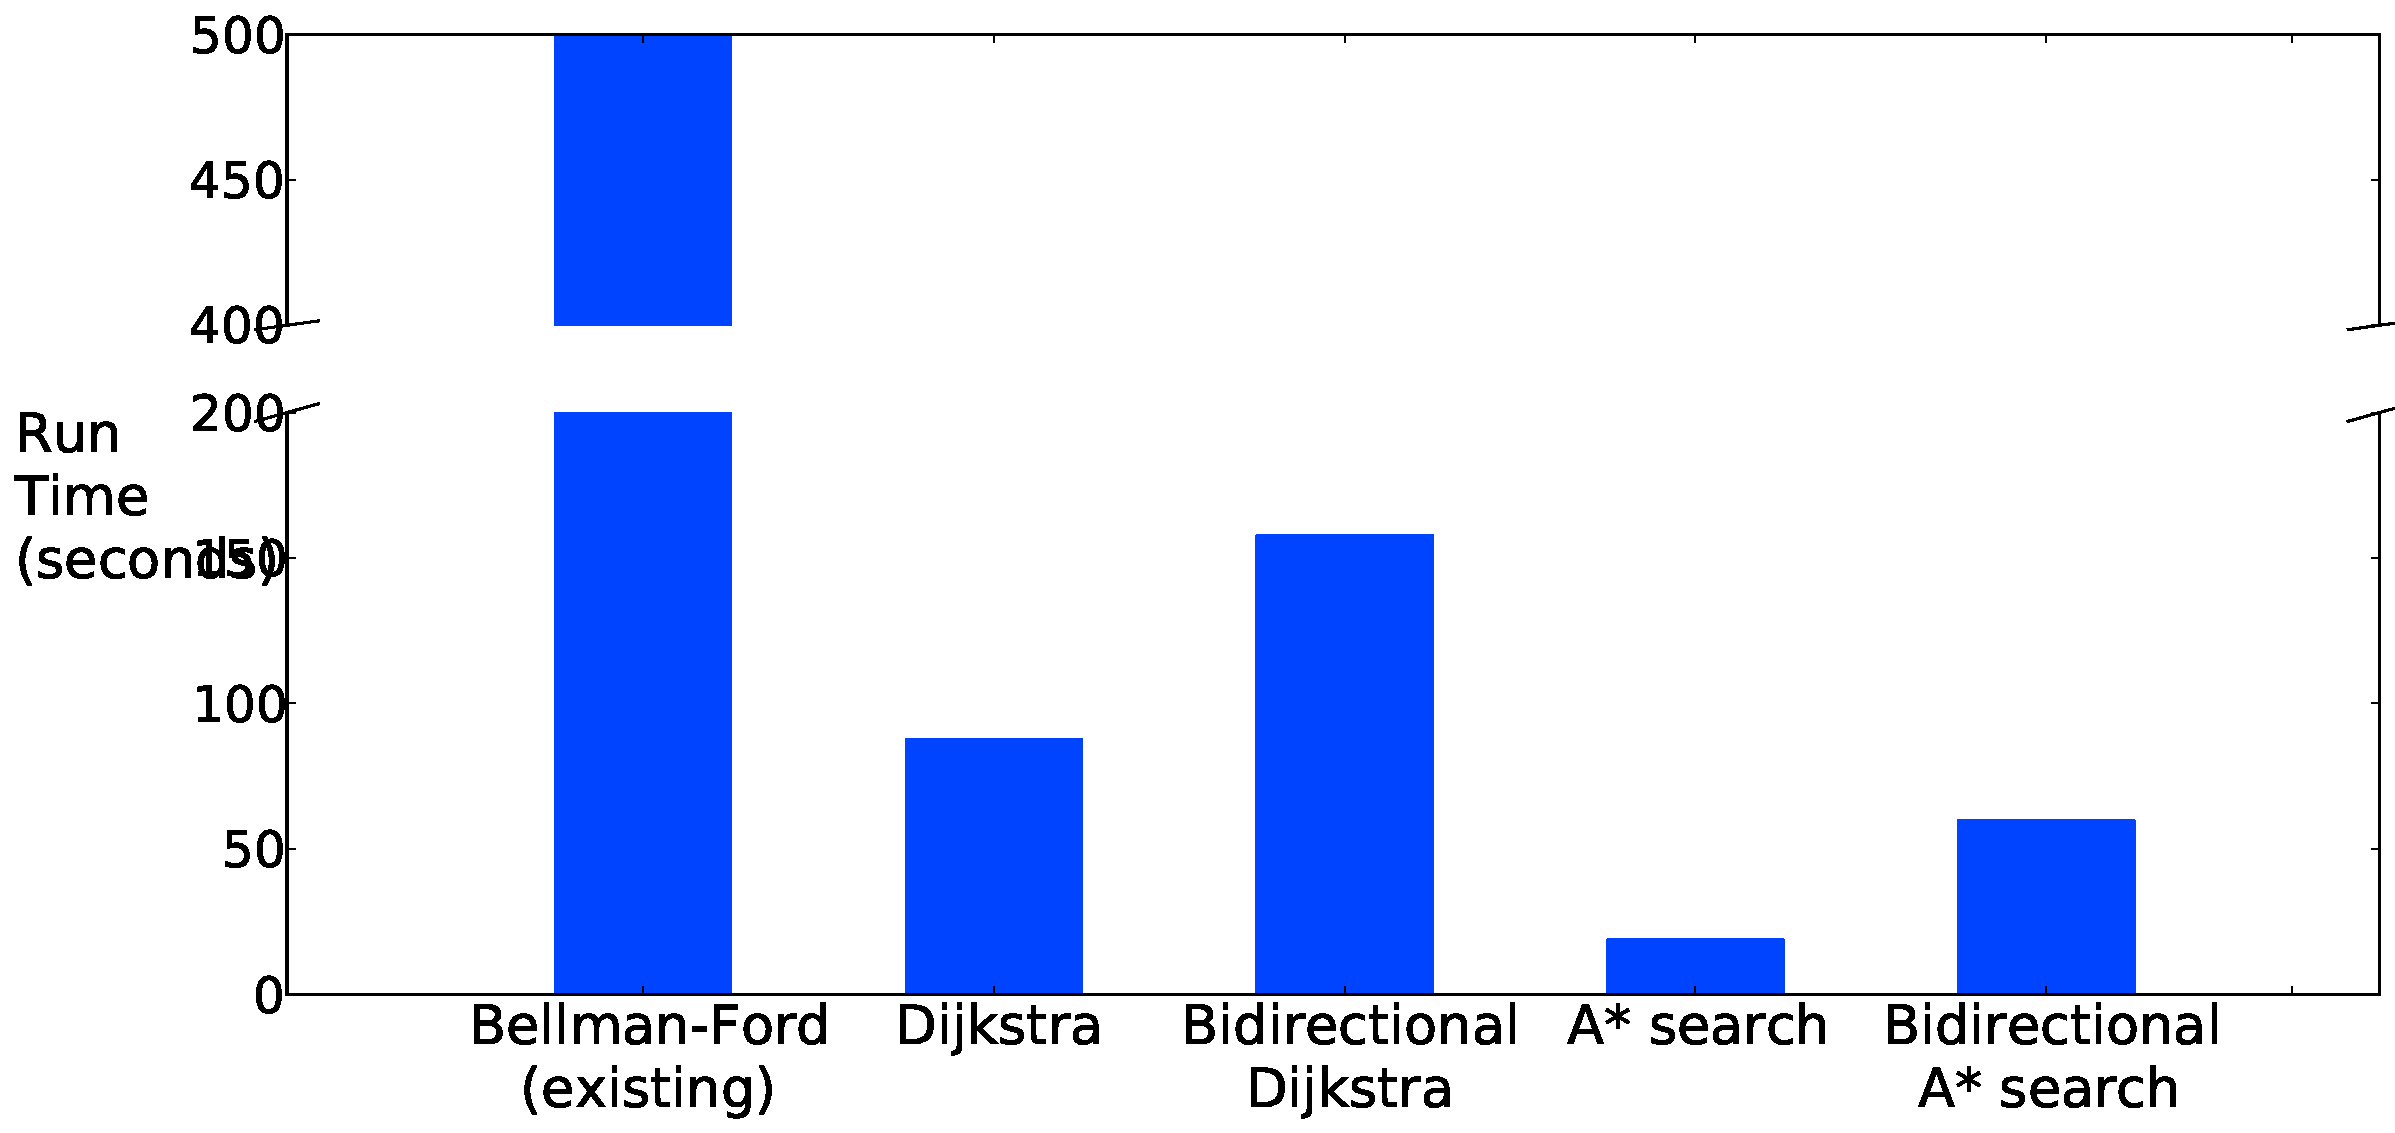
\includegraphics[width=\linewidth]{img/runtime}
                \end{figure}
                \begin{figure}
                    \centering
                    {\bfseries \qquad Run times of Dijkstra's algorithm run times\\ \qquad using different priority queues}
                    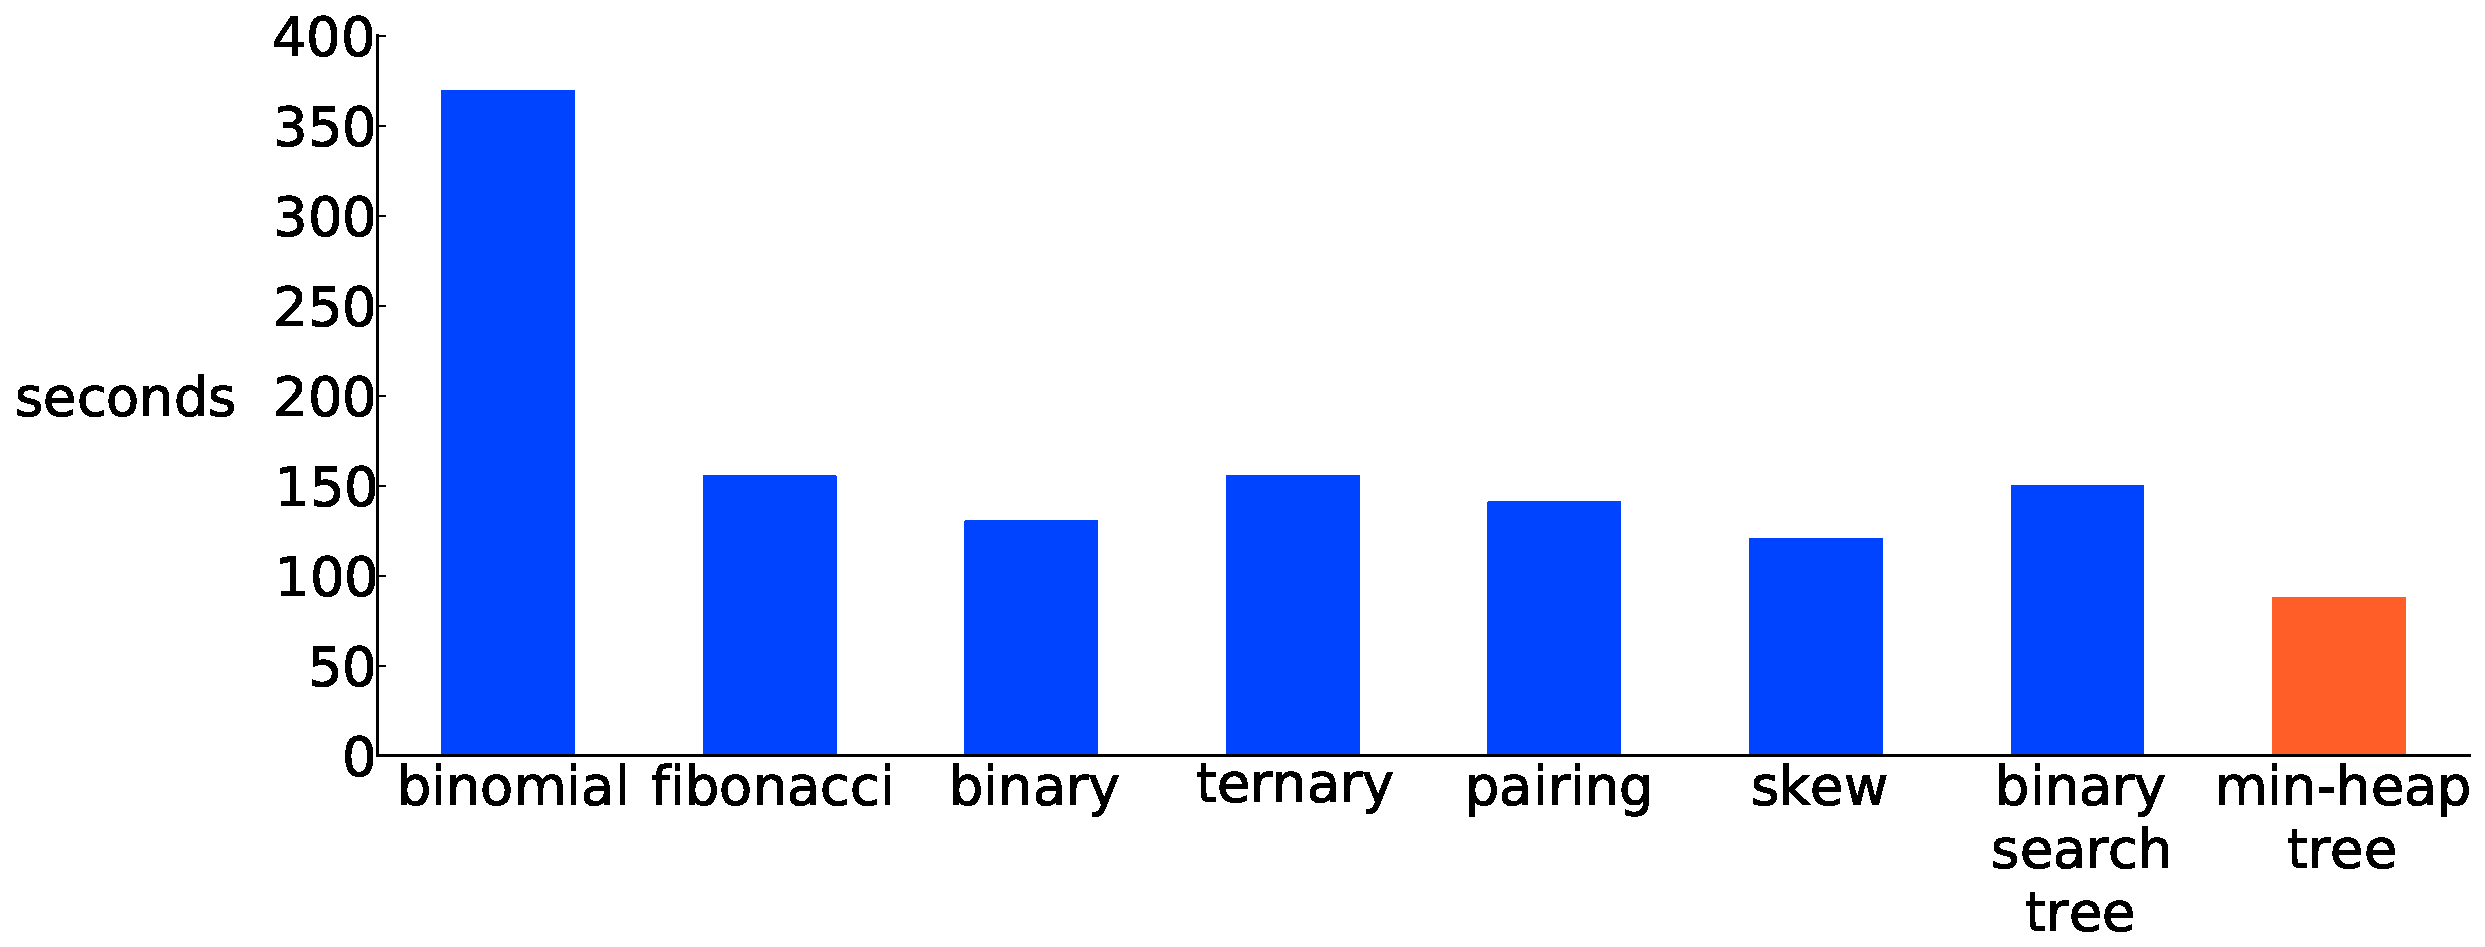
\includegraphics[width=\linewidth]{img/pq_runtime}
                \end{figure}
                \begin{figure}
                    \centering
                    {\bfseries \qquad Run times of A* search using avoiding\\ \qquad shortest path calculation strategies}
                    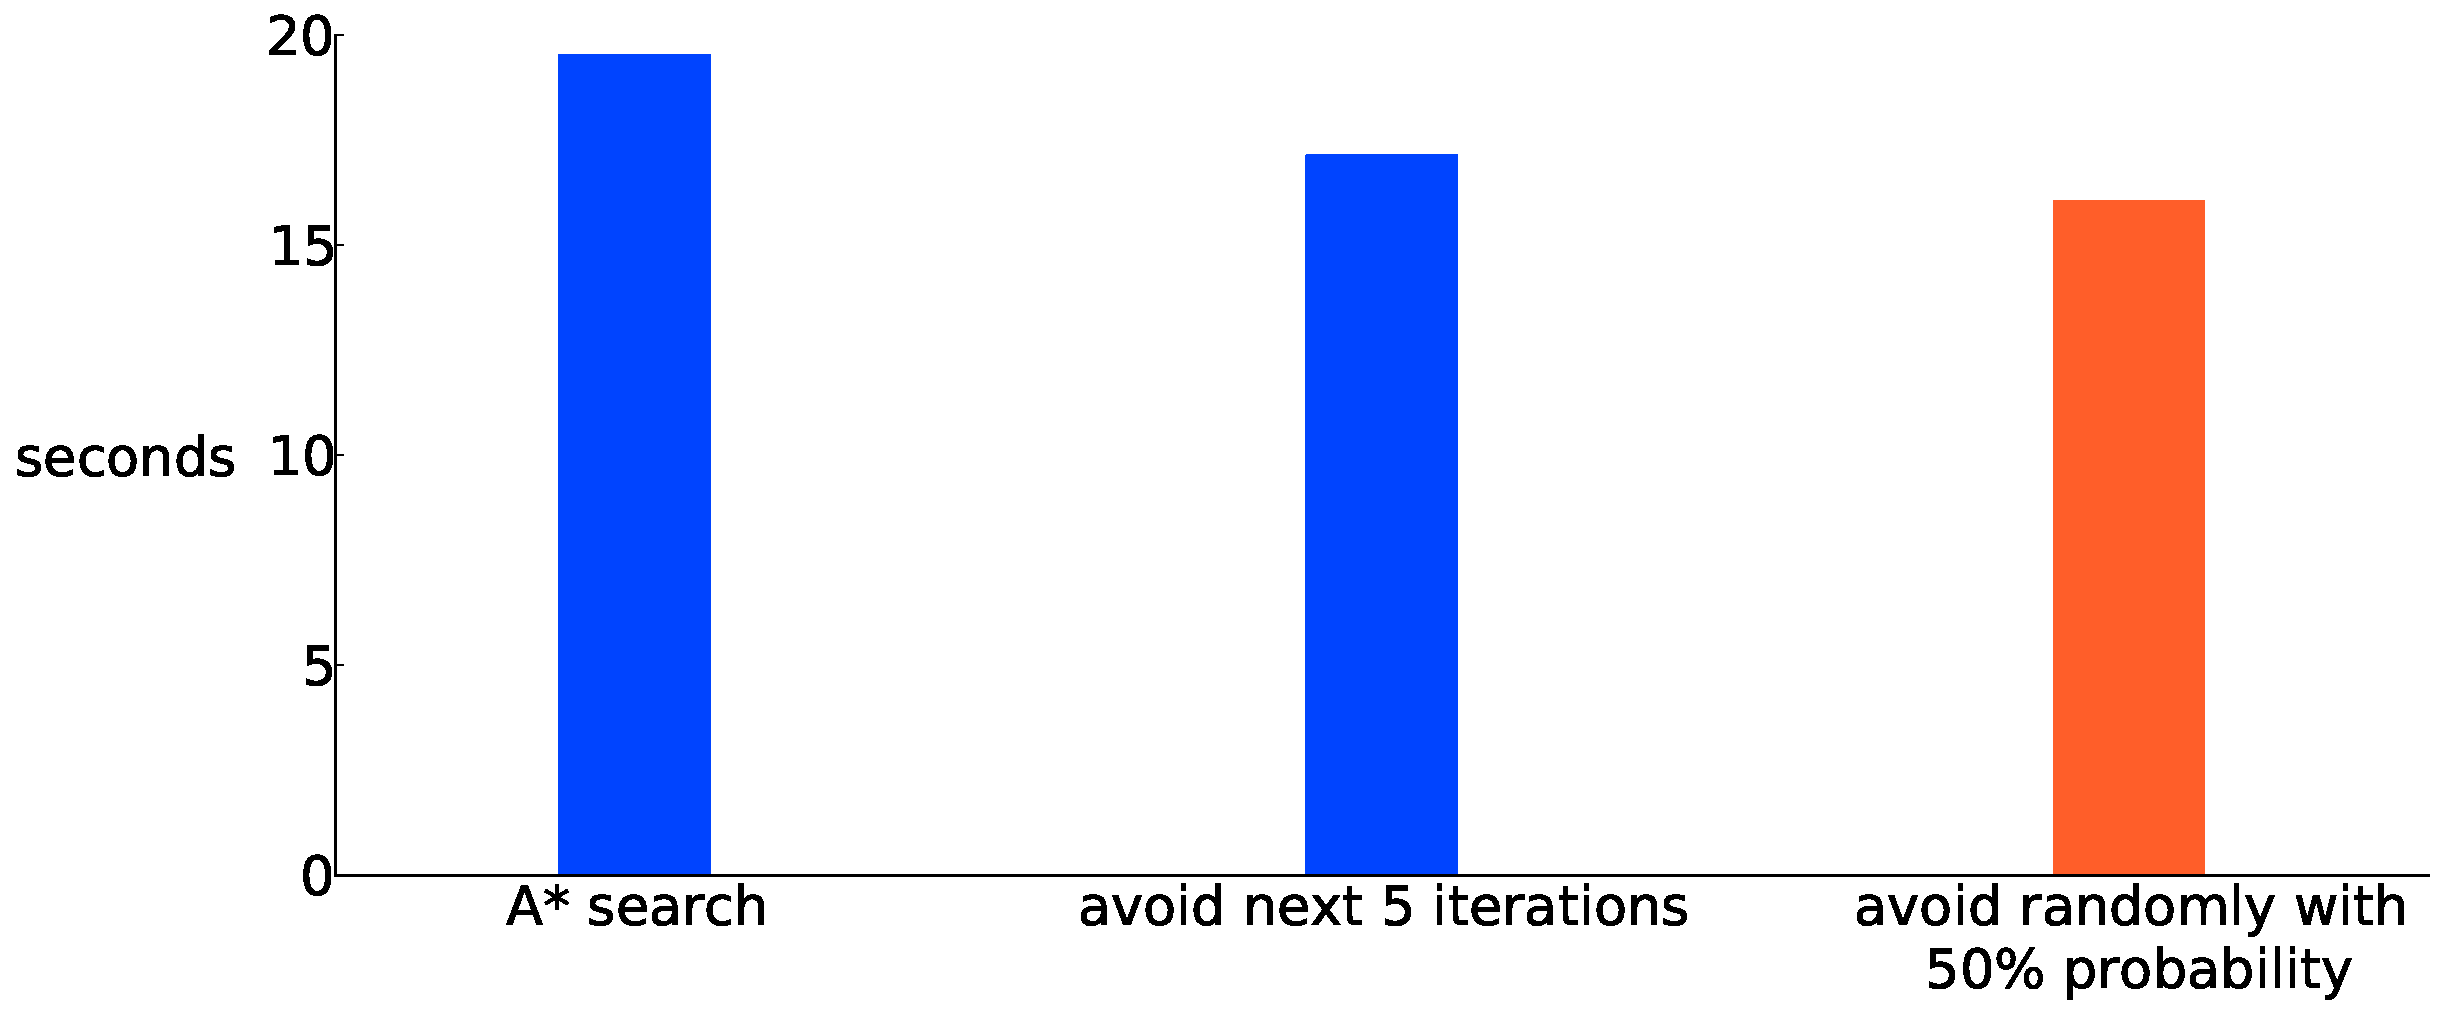
\includegraphics[width=\linewidth]{img/random_runtime}
                \end{figure}
            \end{block}

            \begin{block}{Conclusions}
                \begin{itemize}
                    \item best performance : A* search algorithm with random skipping strategy
                \end{itemize}
            \end{block}

        \end{column}
    \end{columns}
\end{frame}





\end{document}
